\documentclass[class=article, crop=false]{standalone}
\usepackage[subpreambles=false]{standalone}
\usepackage{import}
% Options for packages loaded elsewhere
\PassOptionsToPackage{unicode}{hyperref}
\PassOptionsToPackage{hyphens}{url}


\usepackage{amsmath,amssymb}
\usepackage{lmodern}
\usepackage{iftex}
\ifPDFTeX
  \usepackage[T1]{fontenc}
  \usepackage[utf8]{inputenc}
  \usepackage{textcomp} % provide euro and other symbols
\else % if luatex or xetex
  \usepackage{unicode-math}
  \defaultfontfeatures{Scale=MatchLowercase}
  \defaultfontfeatures[\rmfamily]{Ligatures=TeX,Scale=1}
\fi
% Use upquote if available, for straight quotes in verbatim environments
\IfFileExists{upquote.sty}{\usepackage{upquote}}{}
\IfFileExists{microtype.sty}{% use microtype if available
  \usepackage[]{microtype}
  \UseMicrotypeSet[protrusion]{basicmath} % disable protrusion for tt fonts
}{}
\makeatletter
\@ifundefined{KOMAClassName}{% if non-KOMA class
  \IfFileExists{parskip.sty}{%
    \usepackage{parskip}
  }{% else
    \setlength{\parindent}{0pt}
    \setlength{\parskip}{6pt plus 2pt minus 1pt}}
}{% if KOMA class
  \KOMAoptions{parskip=half}}
\makeatother
\usepackage{xcolor}
\usepackage[margin=1in]{geometry}
\usepackage{color}
\usepackage{fancyvrb}
\newcommand{\VerbBar}{|}
\newcommand{\VERB}{\Verb[commandchars=\\\{\}]}
\DefineVerbatimEnvironment{Highlighting}{Verbatim}{commandchars=\\\{\}}
% Add ',fontsize=\small' for more characters per line
\usepackage{framed}
\definecolor{shadecolor}{RGB}{248,248,248}
\newenvironment{Shaded}{\begin{snugshade}}{\end{snugshade}}
\newcommand{\AlertTok}[1]{\textcolor[rgb]{0.94,0.16,0.16}{#1}}
\newcommand{\AnnotationTok}[1]{\textcolor[rgb]{0.56,0.35,0.01}{\textbf{\textit{#1}}}}
\newcommand{\AttributeTok}[1]{\textcolor[rgb]{0.77,0.63,0.00}{#1}}
\newcommand{\BaseNTok}[1]{\textcolor[rgb]{0.00,0.00,0.81}{#1}}
\newcommand{\BuiltInTok}[1]{#1}
\newcommand{\CharTok}[1]{\textcolor[rgb]{0.31,0.60,0.02}{#1}}
\newcommand{\CommentTok}[1]{\textcolor[rgb]{0.56,0.35,0.01}{\textit{#1}}}
\newcommand{\CommentVarTok}[1]{\textcolor[rgb]{0.56,0.35,0.01}{\textbf{\textit{#1}}}}
\newcommand{\ConstantTok}[1]{\textcolor[rgb]{0.00,0.00,0.00}{#1}}
\newcommand{\ControlFlowTok}[1]{\textcolor[rgb]{0.13,0.29,0.53}{\textbf{#1}}}
\newcommand{\DataTypeTok}[1]{\textcolor[rgb]{0.13,0.29,0.53}{#1}}
\newcommand{\DecValTok}[1]{\textcolor[rgb]{0.00,0.00,0.81}{#1}}
\newcommand{\DocumentationTok}[1]{\textcolor[rgb]{0.56,0.35,0.01}{\textbf{\textit{#1}}}}
\newcommand{\ErrorTok}[1]{\textcolor[rgb]{0.64,0.00,0.00}{\textbf{#1}}}
\newcommand{\ExtensionTok}[1]{#1}
\newcommand{\FloatTok}[1]{\textcolor[rgb]{0.00,0.00,0.81}{#1}}
\newcommand{\FunctionTok}[1]{\textcolor[rgb]{0.00,0.00,0.00}{#1}}
\newcommand{\ImportTok}[1]{#1}
\newcommand{\InformationTok}[1]{\textcolor[rgb]{0.56,0.35,0.01}{\textbf{\textit{#1}}}}
\newcommand{\KeywordTok}[1]{\textcolor[rgb]{0.13,0.29,0.53}{\textbf{#1}}}
\newcommand{\NormalTok}[1]{#1}
\newcommand{\OperatorTok}[1]{\textcolor[rgb]{0.81,0.36,0.00}{\textbf{#1}}}
\newcommand{\OtherTok}[1]{\textcolor[rgb]{0.56,0.35,0.01}{#1}}
\newcommand{\PreprocessorTok}[1]{\textcolor[rgb]{0.56,0.35,0.01}{\textit{#1}}}
\newcommand{\RegionMarkerTok}[1]{#1}
\newcommand{\SpecialCharTok}[1]{\textcolor[rgb]{0.00,0.00,0.00}{#1}}
\newcommand{\SpecialStringTok}[1]{\textcolor[rgb]{0.31,0.60,0.02}{#1}}
\newcommand{\StringTok}[1]{\textcolor[rgb]{0.31,0.60,0.02}{#1}}
\newcommand{\VariableTok}[1]{\textcolor[rgb]{0.00,0.00,0.00}{#1}}
\newcommand{\VerbatimStringTok}[1]{\textcolor[rgb]{0.31,0.60,0.02}{#1}}
\newcommand{\WarningTok}[1]{\textcolor[rgb]{0.56,0.35,0.01}{\textbf{\textit{#1}}}}
\usepackage{longtable,booktabs,array}
\usepackage{calc} % for calculating minipage widths
% Correct order of tables after \paragraph or \subparagraph
\usepackage{etoolbox}
\makeatletter
\patchcmd\longtable{\par}{\if@noskipsec\mbox{}\fi\par}{}{}
\makeatother
% Allow footnotes in longtable head/foot
\IfFileExists{footnotehyper.sty}{\usepackage{footnotehyper}}{\usepackage{footnote}}
\makesavenoteenv{longtable}
\usepackage{graphicx}
\makeatletter
\def\maxwidth{\ifdim\Gin@nat@width>\linewidth\linewidth\else\Gin@nat@width\fi}
\def\maxheight{\ifdim\Gin@nat@height>\textheight\textheight\else\Gin@nat@height\fi}
\makeatother
% Scale images if necessary, so that they will not overflow the page
% margins by default, and it is still possible to overwrite the defaults
% using explicit options in \includegraphics[width, height, ...]{}
\setkeys{Gin}{width=\maxwidth,height=\maxheight,keepaspectratio}
% Set default figure placement to htbp
\makeatletter
\def\fps@figure{htbp}
\makeatother
\setlength{\emergencystretch}{3em} % prevent overfull lines
\providecommand{\tightlist}{%
  \setlength{\itemsep}{0pt}\setlength{\parskip}{0pt}}
\setcounter{secnumdepth}{-\maxdimen} % remove section numbering
\ifLuaTeX
\usepackage[bidi=basic]{babel}
\else
\usepackage[bidi=default]{babel}
\fi
\babelprovide[main,import]{ngerman}
% get rid of language-specific shorthands (see #6817):
\let\LanguageShortHands\languageshorthands
\def\languageshorthands#1{}
\ifLuaTeX
  \usepackage{selnolig}  % disable illegal ligatures
\fi
\IfFileExists{bookmark.sty}{\usepackage{bookmark}}{\usepackage{hyperref}}
\IfFileExists{xurl.sty}{\usepackage{xurl}}{} % add URL line breaks if available
\urlstyle{same} % disable monospaced font for URLs
\hypersetup{
  pdftitle={Pendel},
  pdfauthor={Milena Mensching Justus Weyers},
  pdflang={de},
  hidelinks,
  pdfcreator={LaTeX via pandoc}}

\title{Pendel}
\author{Milena Mensching Justus Weyers}
\date{2022-12-06}

\begin{document}


\hypertarget{versuch-1}{%
\section{Versuch 1}\label{versuch-1}}

\hypertarget{ziel}{%
\subsection{Ziel}\label{ziel}}

Bestimmung der Erdbeschleunigung \(g\). Dafür soll ein Pendel verwendet
werden. Dafür wird der Zusammenhang der Schwingungsdauer (Periodendauer)
\(T\) mit der Pendellänge \(L\) und der Erdbeschleunigung \(g\)
verwendet. Es gilt: \[T(L,g) = 2\pi \sqrt{\frac{L}{g}}\] In diesem
Versuch soll \(L\) bekannt sein und \(g\) untersucht werden.

\begin{figure}
\centering
\includegraphics[width=\textwidth,height=0.4\textheight]{Bilder/Wirkende Kräfte.jpeg}
\caption{Wirkende Kräfte}
\end{figure}

Der genannte Zusammenhang ergibt sich aus der Eigenschaft eines
Fadenpendels nach einer kleinen Auslenkung \(x\) harmonisch zu
schwingen. Die der Auslenkung entgegenwirkende Kraft, die Rückstellkraft
\(F_{Rück}\), ist proportional und entgegengesetzt zu \(x\). Sie ist die
resultierende Kraft aus der Gewichtskraft des Massenstücks am Pendel
(der Faden wird als masselos angenommen) und der Zentripetalkraft
(Zugkraft, durch den Faden in Richtung des
Rotations-/Befestigungspunktes). Mit einer Kleinwinkelannäherung gilt
für \(F_{Rück}\) folgender Zusammenhang:
\begin{equation}\label{Pendel:Rueck}
F_{Rück} = m * \ddot{x} = -\frac{g}{l}*m*x
\end{equation} Werden neben der Luftreibung auch andere, dem System
``Fadenpendel'' Energie entnehmende Effekte verachlässigt, handelt es
sich bei dem Pendel und der nun periodisch stattindenden Umwandlung von
potentieller Energie, am Punkte der Maximalauslenkung, in kinetische
Energie, am Punkt der maximalen Geschwindigkeit, um einen harmonischen
Oszillator. Die Auslenkung \(x\) aus Formel \label{Pendel:Ruek} ist
dabei zeitabhängig und kann wie alle harmonischen Schwingungen duch
Amplitude \(\hat{x}\) und Winkelgeschwindigkeit \(\omega\) beschrieben
werden: \begin{equation}\label{Pendel:Schwingung}
  x(t,\omega) = \hat{x} \cdot cos(\omega \cdot t)
\end{equation} Die Winkelgeschwindigkeit ist dabei abhängig von
Erdbeschleunigung und Pendellänge, vergleiche Formel \ref{Pendel:Rueck},
sie beträgt \(\omega=\sqrt{\frac{g}{l}}\). Über diese
Winkelgeschwindigkeit kann mit dem Zusammenhang \(T=2\pi\omega\) die
Periodendauer für einen Pendelschlag bestimmt werden als:
\begin{equation}\label{Pendel:Periodendauer}
T(L) = 2\pi \sqrt{\frac{L}{g}}
\end{equation}

\hypertarget{materialien}{%
\subsection{Materialien}\label{materialien}}

\begin{itemize}
\tightlist
\item
  Stativ
\item
  Pendel aus Angelschnur und Metallzylinder
\item
  Maßband
\item
  Messschieber
\item
  Klebeband
\item
  Stoppuhr
\item
  Berechnungen finden in Excel und R statt
\end{itemize}

\hypertarget{versuchsaufbau}{%
\subsection{Versuchsaufbau}\label{versuchsaufbau}}

\begin{itemize}
\tightlist
\item
  Aufstellung des Stativs, Befestigung oberhalb des Tisches
\item
  Befestigung des Maßbandes am Stativ mit Hilfe von Klebeband
\end{itemize}

\begin{figure}
\centering
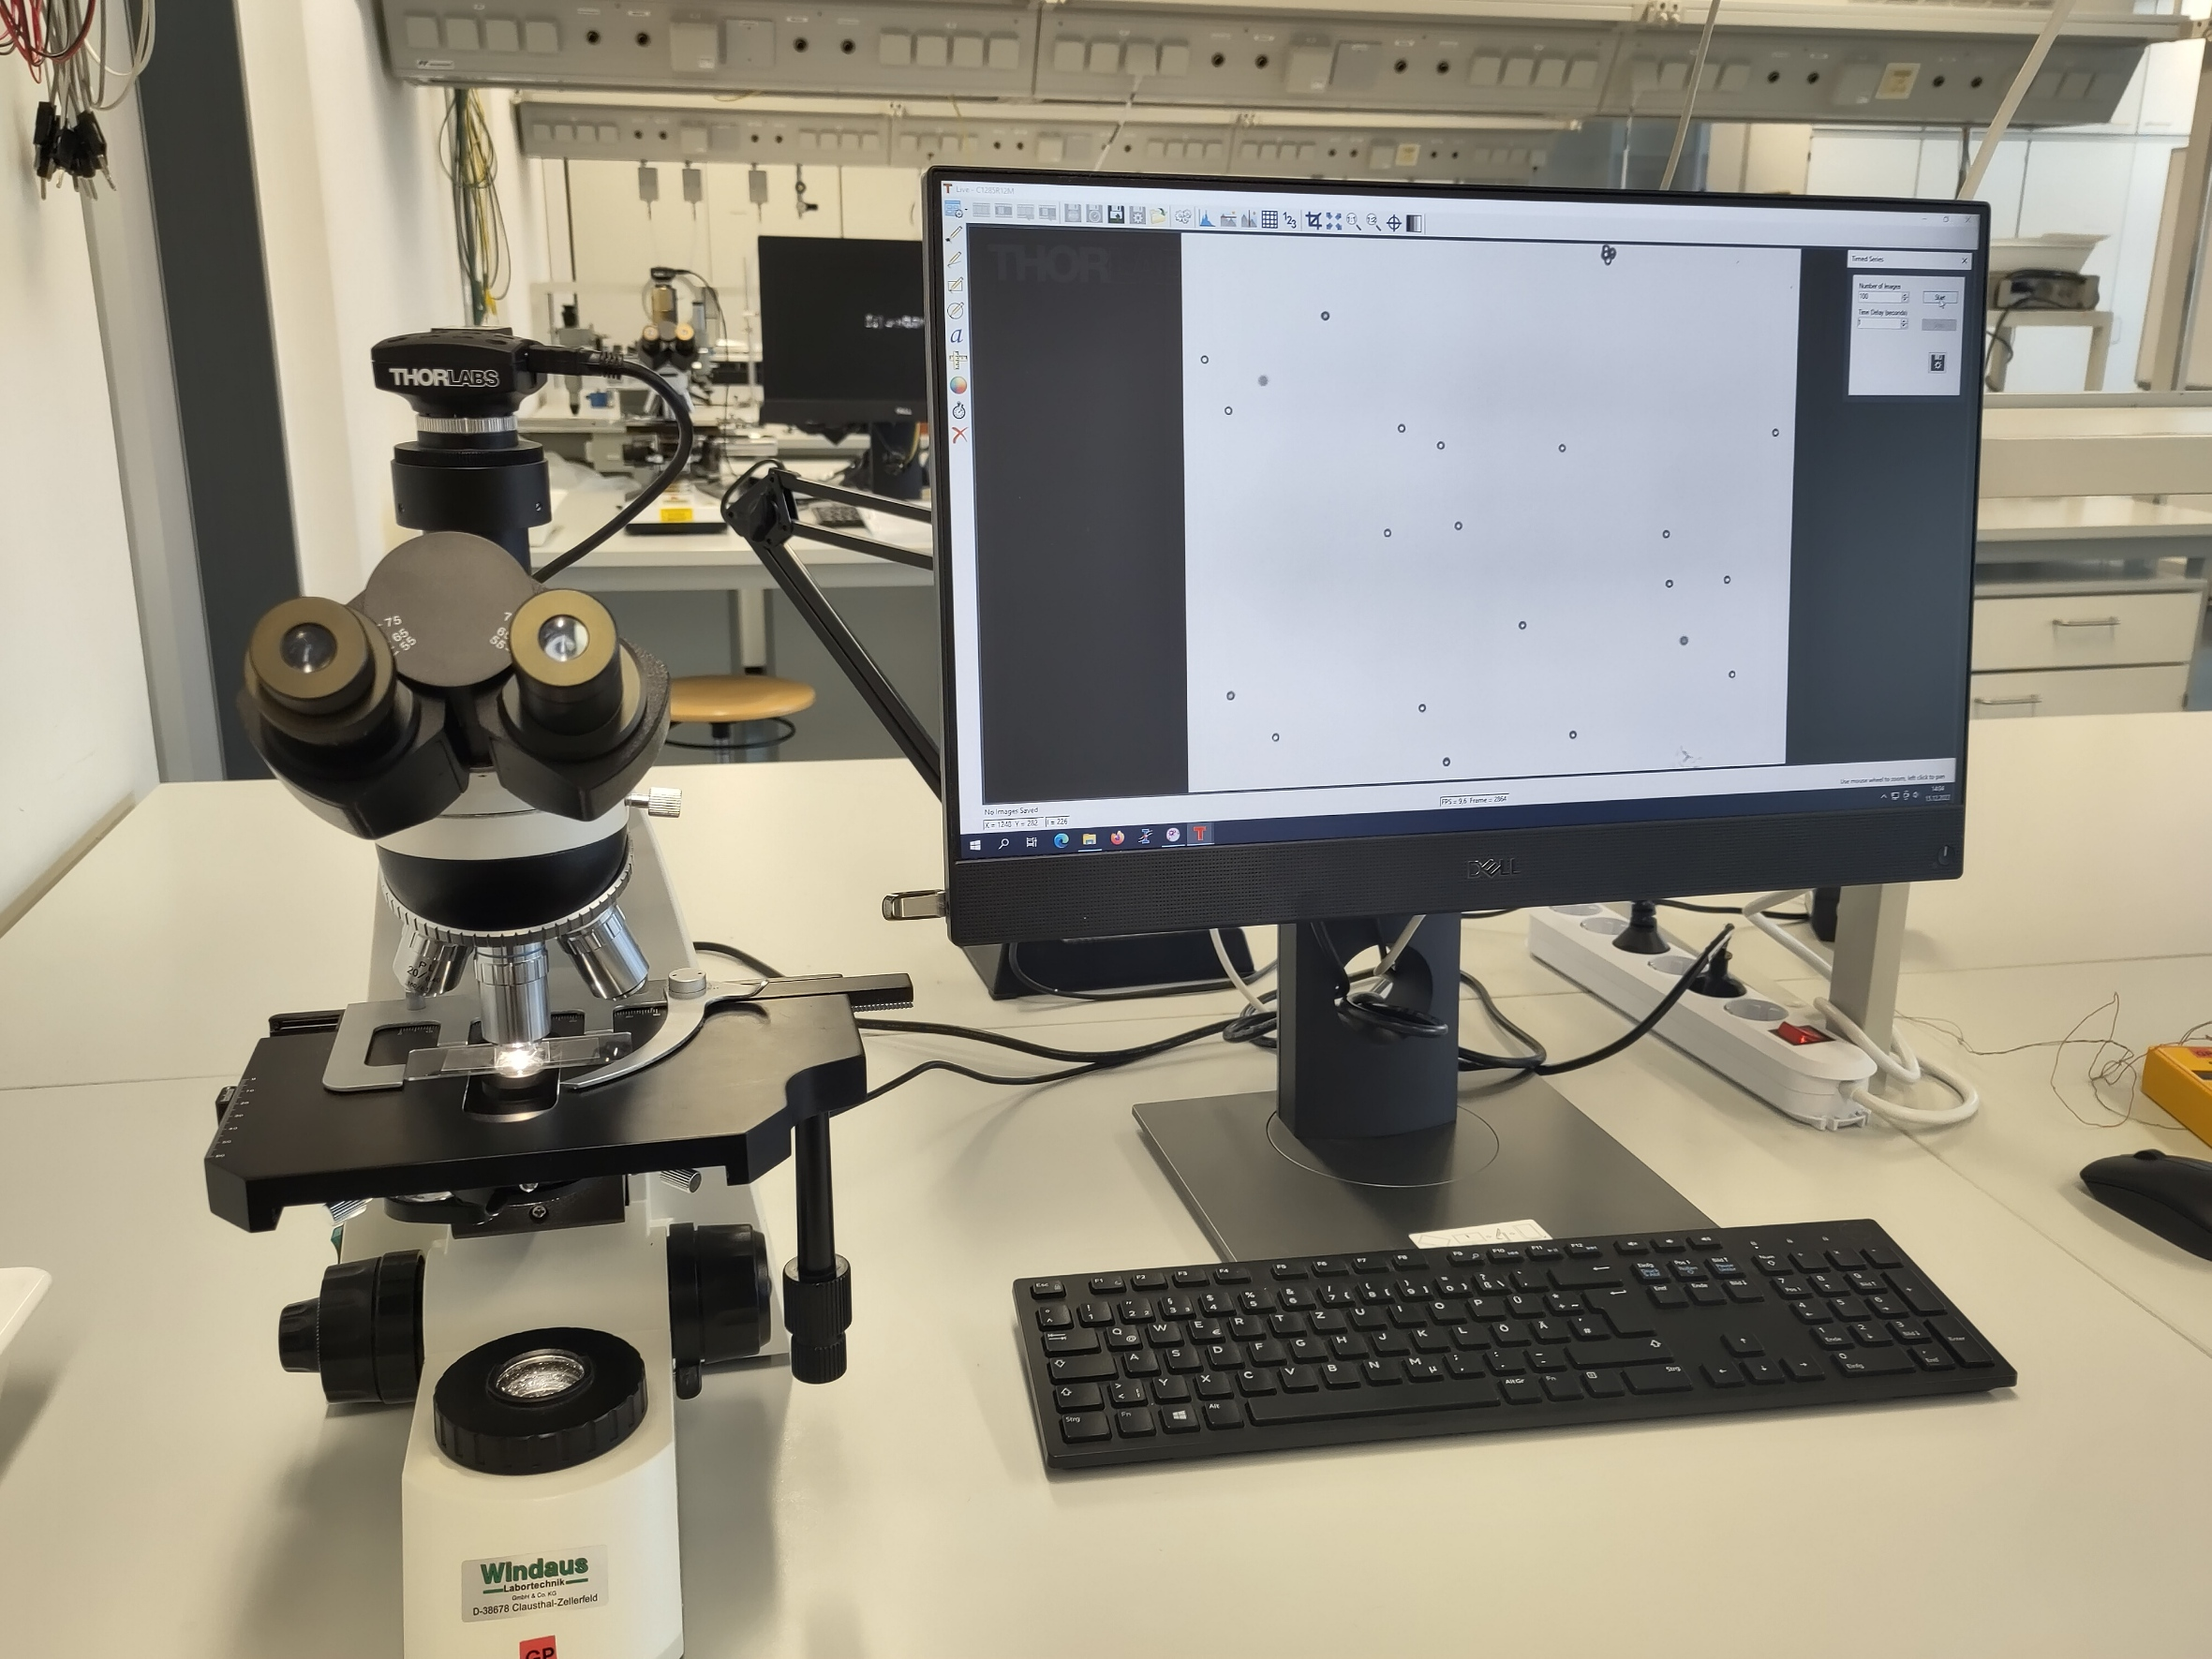
\includegraphics[width=\textwidth,height=0.3\textheight]{Bilder/Versuchsaufbau.png}
\caption{Versuchsaufbau}
\end{figure}

\hypertarget{durchfuxfchrung}{%
\subsection{Durchführung}\label{durchfuxfchrung}}

Nach dem Versuchsaufbau wird mit der Versuchsdurchführung begonnen. Dazu
wird die Pendellänge vermessen, indem am Maßband die Position des
Drehpunktes (L1) und die Position der Oberkante des Zylindergewichtes
abgelesen werden (L2). Die Höhe des Zylindergewichtes wird mit einem
Messschieber vermessen (L3).

Im Anschluss wird die Periodendauer für diese Pendellänge bestimmt. Dazu
wird das Pendel aus der Ruheposition ausgelenkt und nach ein paar
Pendelschlägen mit der Zeitmessung begonnen. Die Zeit wird beim
Durchgang durch den Ort der maximalen Geschwindigkeit sowohl gestartet
als auch gestoppt, um die Reaktionszeit möglichst kurz zu halten. Es
werden insgesamt 5 Messungen durchgeführt um einen Mittelwert bilden zu
können.

\hypertarget{fehlerquellen}{%
\subsection{Fehlerquellen}\label{fehlerquellen}}

Beim Auslenken des Pendels gibt es \textbf{unregelmäßige Bewegungen
(Wackeln)}, die entgegen der Pendelbahn laufen.

Beim Abmessen der Pendellänge ist der \textbf{personenbezogene
Ablesefehler} zu erwähnen. Diesen versuchten wir weitestgehend zu
eliminieren, indem nur eine Person eine vollständige Datenreihe aufnahm.

Außerdem verlängert die \textbf{Reaktionszeit} sowohl bei Start als auch
bei Stopp der Messung tendenziell die gemessene Periodendauer. Um diesen
Fehler möglichst gering zu halten, wurden zehn Periodendurchläufe
gemessen und die Periodendauer danach gemittelt. Auch hier nahm nur eine
Person die Datenreihe auf, um die Reaktionszeit ähnlich zu halten.

Folgende Annahmen mussten darüber hinaus getroffen werden:

\begin{itemize}
\tightlist
\item
  Bewegung des Pendelkörpers und des Fadens verläuft reibungsfrei
\item
  Masse des Fadens wird vernachlässigt
\item
  Der Pendelkörper wird nur um eine kleine Strecke ausgelenkt
\item
  Die Angelschnur ist inelastisch
\end{itemize}

\hypertarget{messungen}{%
\subsection{Messungen}\label{messungen}}

Im Laufe von Versuch 1 wurden folgende Messwerte aufgenommen, auf die
sich in der folgenden Auswertung bezogen wird:

\begin{longtable}[]{@{}lr@{}}
\caption{Messwerte aus Versuch 1}\tabularnewline
\toprule()
Messgröße & Wert \\
\midrule()
\endfirsthead
\toprule()
Messgröße & Wert \\
\midrule()
\endhead
L1: Position Drehpunkt {[}cm{]} & 4.00 \\
L2: Position Fadenende {[}cm{]} & 88.50 \\
L3: Höhe Zylinder {[}cm{]} & 5.87 \\
10-Periodendauer {[}s{]} & 18.75 \\
10-Periodendauer {[}s{]} & 18.72 \\
10-Periodendauer {[}s{]} & 18.85 \\
10-Periodendauer {[}s{]} & 18.85 \\
10-Periodendauer {[}s{]} & 18.72 \\
\bottomrule()
\end{longtable}

Die fünf Punkte ``10-Periodendauer {[}s{]}'' sind die fünfmal
durchgeführten Messungen, aus denen der Mittelwert berechnet werden
soll.

\hypertarget{auswertung}{%
\subsection{Auswertung}\label{auswertung}}

\hypertarget{pendelluxe4nge-l-und-unsicherheit-u_l}{%
\subsubsection{\texorpdfstring{Pendellänge L und Unsicherheit
\(u_L\)}{Pendellänge L und Unsicherheit u\_L}}\label{pendelluxe4nge-l-und-unsicherheit-u_l}}

Die Pendellänge \(L\) wird bestimmt, indem die Differenz von \(L_1\) und
\(L_2\) berechnet wird, siehe Tabelle im Abschnitt \textit{Messungen}.
Es wird auch darauf geachtet, die Distanz von der Pendeloberkante bis
zum Massenschwerpunkt des Pendels dazuzurechnen. Dafür wird die
Massenverteilung in dem Metallzylinder-Gewicht als homogen angenommen.
Die zu der Fadenlänge zu addierende Länge entspricht dann der halben
Zylinderhöhe \(L_3\). Der Bestwert der errechneten Pendellänge \(L\)
beträgt dann:

\begin{align*}
L&= L_2-L_1+\frac{L_{3}}{2}\\
 &=0,885m-0,04m+\frac{0,0587}{2}m\\
 &=0,87435m.\\
\end{align*}

\begin{Shaded}
\begin{Highlighting}[]
\CommentTok{\# Bestwert Pendellänge in Metern}
\FloatTok{0.885{-}0.04+0.0587}\SpecialCharTok{/}\DecValTok{2}
\end{Highlighting}
\end{Shaded}

\begin{verbatim}
## [1] 0.87435
\end{verbatim}

Die Unsicherheit der Pendellänge setzt sich aus den zu \(L_1\), \(L_2\)
und \(L_3\) gehörigen Messunsicherheiten zusammen:
\begin{equation}\label{Pendel:U_L}
\begin{split}
u_L&= \sqrt{(\frac{\partial L}{\partial L_2} \cdot u_{Massband})^2+(\frac{\partial L}{\partial L_1} \cdot u_{Massband})^2+(\frac{\partial L}{\partial L_{3}} \cdot u_{Messchieber})^2}\\
&= \sqrt{u_{Massband}^2*(\frac{\partial L}{\partial L_2}^2+\frac{\partial L}{\partial L_1}^2)+(\frac{\partial L}{\partial L_{3}}*u_{Messschieber})^2}\\
&=\sqrt{(\frac{10^{-3}m}{2\sqrt{6}})^2*(1^2+(-1)^2)+(0,5*\frac{10^{-4}m}{2\sqrt{6}})^2}\\
&\approx 0,29 \cdot 10^{-4}m\\
\end{split}
\end{equation}

Mit:

\begin{itemize}
  \item Messunsicherheit des Maßbandes: $u_{Massband}=\frac{10^{-3}m}{2\sqrt{6}}$
  \item Messunsicherheit des Messschiebers: $u_{Messschieber}=\frac{10^{-4}m}{2\sqrt{6}}$
\end{itemize}

\begin{Shaded}
\begin{Highlighting}[]
\CommentTok{\# Berechnung von u\_L in R}
\FunctionTok{sqrt}\NormalTok{(}\DecValTok{2}\SpecialCharTok{*}\NormalTok{(((}\DecValTok{10}\SpecialCharTok{**{-}}\DecValTok{3}\NormalTok{)}\SpecialCharTok{/}\NormalTok{(}\DecValTok{2}\SpecialCharTok{*}\FunctionTok{sqrt}\NormalTok{(}\DecValTok{6}\NormalTok{)))}\SpecialCharTok{**}\DecValTok{2}\NormalTok{)}\SpecialCharTok{+}\NormalTok{((}\DecValTok{10}\SpecialCharTok{**{-}}\DecValTok{4}\NormalTok{)}\SpecialCharTok{/}\NormalTok{(}\DecValTok{2}\SpecialCharTok{*}\FunctionTok{sqrt}\NormalTok{(}\DecValTok{6}\NormalTok{)))}\SpecialCharTok{**}\DecValTok{2}\NormalTok{)}
\end{Highlighting}
\end{Shaded}

\begin{verbatim}
## [1] 0.0002893959
\end{verbatim}

Damit beträgt die Pendellänge für Versuch 1
\(L = (0,87435 \pm 0.00029)m\).

\hypertarget{periodendauer-t-und-unsicherheit-u_t}{%
\subsubsection{\texorpdfstring{Periodendauer T und Unsicherheit
\(u_T\)}{Periodendauer T und Unsicherheit u\_T}}\label{periodendauer-t-und-unsicherheit-u_t}}

Als Zeit für zehn Perioden \(T_{10T}\) in Sekunden wird der Mittelwert
der fünf Messungen aus der Tabelle im Abschnitt \textit{Messungen}
berechnet.

\begin{Shaded}
\begin{Highlighting}[]
\NormalTok{T\_10T }\OtherTok{\textless{}{-}} \FunctionTok{mean}\NormalTok{(Werte[}\DecValTok{4}\SpecialCharTok{:}\DecValTok{8}\NormalTok{])}
\NormalTok{T\_10T}
\end{Highlighting}
\end{Shaded}

\begin{verbatim}
## [1] 18.778
\end{verbatim}

Die mittlere Periodendauer \(T\) in Sekunden wird bestimmt, indem
\(T_{10T}\) durch die Anzahl von Perioden \(n=10\) geteilt wird.

\[T_{10T} = n*T \Leftrightarrow T = \frac{18,778s}{10}=1.8778s\]

Die Messunsicherheit der digitalen Stoppuhr \(u_{Stoppuhr}\) ist die
Unsicherheit für \(T_{10T}\). Deren kleinste ablesbare Größenordnung
waren sind Millisekunden. Damit folgt für \(u_{10T}\):
\(u_{10T}= \frac{a}{2\sqrt{3}} = \frac{0,01s}{2\sqrt{3}} \approx 0,0029s\).

Die Unsicherheit der Periodendauer \(u_T\) ist für zehn Perioden dann
ein Zehntel der Messunsicherheit für zehn Perioden, also
\(u_T=0.00029s\).

Damit ergibt sich die Periodendauer als: \(T=(1.87780 \pm 0.00029)s\).

\hypertarget{berechnung-der-erdbeschluxe4unugung-g-und-der-unsicherheit-u_g}{%
\subsubsection{\texorpdfstring{Berechnung der Erdbeschläunugung g und
der Unsicherheit
\(u_g\)}{Berechnung der Erdbeschläunugung g und der Unsicherheit u\_g}}\label{berechnung-der-erdbeschluxe4unugung-g-und-der-unsicherheit-u_g}}

Mit den Bestwerten für die Pendellänge \(L\) und die Periodendauer \(T\)
kann der Bestwert der Erdbeschleunigung \(g\) berechnet werden. In
Formel \ref{Pendel:Periodendauer} eingesetzt ergibt sich mit
\(L = 0,8744m\) und \(T = 1,878s\):

\begin{equation*}
\begin{split}
g&=\frac{4*\pi^2*l}{T^2}\\
\Rightarrow &=\frac{4*\pi^2*0,87435m}{(1,8778s)^2}\\
 &= 9,789182 \frac{m}{s^2} 
\end{split}
\end{equation*}

\begin{Shaded}
\begin{Highlighting}[]
\NormalTok{(}\DecValTok{4}\SpecialCharTok{*}\NormalTok{pi}\SpecialCharTok{**}\DecValTok{2}\SpecialCharTok{*}\FloatTok{0.87435}\NormalTok{)}\SpecialCharTok{/}\NormalTok{(}\FloatTok{1.8778}\SpecialCharTok{**}\DecValTok{2}\NormalTok{)}
\end{Highlighting}
\end{Shaded}

\begin{verbatim}
## [1] 9.789182
\end{verbatim}

Messunsicherheit \(u_g\) der Erdbeschleunigung \(g\): \begin{equation*}
\begin{split}
u_g&=\sqrt{(\frac{\partial g}{\partial T}*u_T)^2+(\frac{\partial g}{\partial l}*u_l)^2}\\
   &=\sqrt{(\frac{-8*\pi^2*l}{T^3}*u_T)^2+(\frac{4*\pi^2}{T^2}*u_l)^2}\\
\Rightarrow &= \sqrt{(\frac{-8\pi^2*(0,87435m)}{(1,8778s)^3}*(0,00029s))^2+(\frac{4\pi^2}{(1,8778s)^2}*(0,00029m))^2}\\
u_g&\approx \pm 0,0044 \frac{m}{s^2}
\end{split}
\end{equation*}

\begin{Shaded}
\begin{Highlighting}[]
\CommentTok{\# Berechnung von u\_g in R}
\FunctionTok{sqrt}\NormalTok{(( (}\SpecialCharTok{{-}}\DecValTok{8}\SpecialCharTok{*}\NormalTok{pi}\SpecialCharTok{**}\DecValTok{2}\SpecialCharTok{*}\FloatTok{0.87435}\NormalTok{)}\SpecialCharTok{/}\NormalTok{(}\FloatTok{1.8778}\NormalTok{)}\SpecialCharTok{**}\DecValTok{3} \SpecialCharTok{*}\FloatTok{0.00029}\NormalTok{)}\SpecialCharTok{**}\DecValTok{2}\SpecialCharTok{+}\NormalTok{( (}\DecValTok{4}\SpecialCharTok{*}\NormalTok{pi}\SpecialCharTok{**}\DecValTok{2}\NormalTok{)}\SpecialCharTok{/}\NormalTok{(}\FloatTok{1.8778}\NormalTok{)}\SpecialCharTok{**}\DecValTok{2} \SpecialCharTok{*}\FloatTok{0.00029}\NormalTok{ )}\SpecialCharTok{**}\DecValTok{2}\NormalTok{)}
\end{Highlighting}
\end{Shaded}

\begin{verbatim}
## [1] 0.004436673
\end{verbatim}

Damit haben wir in Versuch 1 eine Erdbeschleunigung von
\(g=(9,7891 \pm 0,0044)\frac{m}{s^2}\) gemessen.

\hypertarget{interpretation}{%
\subsection{Interpretation}\label{interpretation}}

Der Literaturwert von \(g=9,81\frac{m}{s^2}\) liegt damit nicht im
Fehlerintervall. Eventuell kann in einem Versuch, bei dem die
Pendellänge varriiert wird ein besseres Ergebnis erziehlt werden.

\textit{Vielleicht hier noch 'nen Ast abbrechen.}

\newpage

\hypertarget{versuch-2}{%
\section{Versuch 2}\label{versuch-2}}

Der zweite Versuch läuft analog zum ersten Versuch. Allerdings werden
statt nur einer Messreihe 5 verschiedene - jeweils mit einer anderen
Fadenlänge - gemessen. Um die Pendellängen zu variieren wurde der Faden
für kürzere Fadenlängen mit Klebeband am Zylinder stückchenweise
festgeklebt. Für längere Pendellängen wurden weitere Stücke Angelschnur
an das Pendel geknotet.

\hypertarget{fehlerquellen-1}{%
\subsection{Fehlerquellen}\label{fehlerquellen-1}}

Die Fehlerquellen sind ebenfalls die selben wie beim ersten Versuch.
Allerdings ist hierbei zu bemerken, dass die Reaktioszeit bei kürzeren
Fadenlängen und daraus resultierenden kürzeren Periodendauern
verhältnismäßig zunimmt. Auch von der Bahn abweichende Bewegungen nehmen
bei kürzeren Pendellängen zu. Auch ist nicht unterscuht, wie sich
Klebeband bzw. Knoten im Faden auf das Pendelverhalten auswirken.

\hypertarget{messungen-1}{%
\subsection{Messungen}\label{messungen-1}}

In die zu diesem Versuch gehörigen Werte wurden auch die Messwerte aus
Versuch 1 integriert. Es wurde wieder so verfahren, dass pro Pendellänge
fünf Messungen der Zeit für 10 Perioden gemessen und der Mittelwert
berechnet wurde.

Die Messwerte sind die folgenden:

\begin{longtable}[]{@{}
  >{\raggedright\arraybackslash}p{(\columnwidth - 14\tabcolsep) * \real{0.2632}}
  >{\raggedleft\arraybackslash}p{(\columnwidth - 14\tabcolsep) * \real{0.1053}}
  >{\raggedleft\arraybackslash}p{(\columnwidth - 14\tabcolsep) * \real{0.1053}}
  >{\raggedleft\arraybackslash}p{(\columnwidth - 14\tabcolsep) * \real{0.1053}}
  >{\raggedleft\arraybackslash}p{(\columnwidth - 14\tabcolsep) * \real{0.1053}}
  >{\raggedleft\arraybackslash}p{(\columnwidth - 14\tabcolsep) * \real{0.1053}}
  >{\raggedleft\arraybackslash}p{(\columnwidth - 14\tabcolsep) * \real{0.1053}}
  >{\raggedleft\arraybackslash}p{(\columnwidth - 14\tabcolsep) * \real{0.1053}}@{}}
\toprule()
\begin{minipage}[b]{\linewidth}\raggedright
\end{minipage} & \begin{minipage}[b]{\linewidth}\raggedleft
Versuch 1
\end{minipage} & \begin{minipage}[b]{\linewidth}\raggedleft
Versuch 2
\end{minipage} & \begin{minipage}[b]{\linewidth}\raggedleft
Versuch 3
\end{minipage} & \begin{minipage}[b]{\linewidth}\raggedleft
Versuch 4
\end{minipage} & \begin{minipage}[b]{\linewidth}\raggedleft
Versuch 5
\end{minipage} & \begin{minipage}[b]{\linewidth}\raggedleft
Versuch 6
\end{minipage} & \begin{minipage}[b]{\linewidth}\raggedleft
Versuch 7
\end{minipage} \\
\midrule()
\endhead
L1:Oberes\_Ende\_in\_cm & 4.0000 & 4.0000 & 4.0000 & 4.0000 & 4.0000 &
4.0000 & 4.0000 \\
L2:UnteresEnde\_in\_cm & 88.5000 & 74.3000 & 58.6000 & 46.0000 & 30.3000
& 114.9000 & 148.6000 \\
L3:Zylinderhoehe\_in\_cm & 5.8700 & 5.8700 & 5.8700 & 5.8700 & 5.8700 &
5.8700 & 5.8700 \\
Pendellaenge\_L & 87.4435 & 73.2435 & 57.5435 & 44.9435 & 29.2435 &
113.8435 & 147.5435 \\
Zeit\_fuer\_10-Perioden\_ 1 & 18.7500 & 17.2200 & 15.4700 & 13.4400 &
10.8500 & 21.5000 & 24.3700 \\
Zeit\_fuer\_10-Perioden\_ 2 & 18.7200 & 17.2800 & 15.4400 & 13.5000 &
10.9700 & 21.4400 & 24.4400 \\
Zeit\_fuer\_10-Perioden\_ 3 & 18.8500 & 17.1800 & 15.5000 & 13.5000 &
10.9400 & 21.4400 & 24.4400 \\
Zeit\_fuer\_10-Perioden\_ 4 & 18.8500 & 17.2800 & 15.5600 & 13.5300 &
11.0300 & 21.5000 & 24.4700 \\
Zeit\_fuer\_10-Perioden\_ 5 & 18.7200 & 17.2500 & 15.4400 & 13.5300 &
10.9100 & 21.4700 & 24.7300 \\
10-Perioden\_Mittelwert & 18.7800 & 17.2400 & 15.4800 & 13.5000 &
10.9400 & 21.4700 & 24.4900 \\
\bottomrule()
\end{longtable}

\hypertarget{auswertung-1}{%
\subsection{Auswertung}\label{auswertung-1}}

\hypertarget{bereits-aus-versuch-1-bekannte-gruxf6uxdfen}{%
\subsubsection{Bereits aus Versuch 1 bekannte
Größen}\label{bereits-aus-versuch-1-bekannte-gruxf6uxdfen}}

Damit sind die Werte für die Pendellänge sowie deren konstante
Unsicherheit \(u_L=0,00029m\), siehe Formel \ref{Pendel:U_L}, bekannt.
Ebenso sind die Werte für die Periodendauer \(T\) bekannt, diese
entsprechen einem Zehntel der Zeit für die gemessenen zehn Perioden. Die
Unsicherheit für T ist auch aus Versuch 1 übernehmbar, diese beträgt
\(u_T = 0,00029s\).

\hypertarget{graphische-darstellung-der-messwerte}{%
\subsubsection{Graphische Darstellung der
Messwerte}\label{graphische-darstellung-der-messwerte}}

Zur Veranschaulichung der Messwerte wird die Periodendauer \(T\) gegen
die Pendellänge aufgetragen:
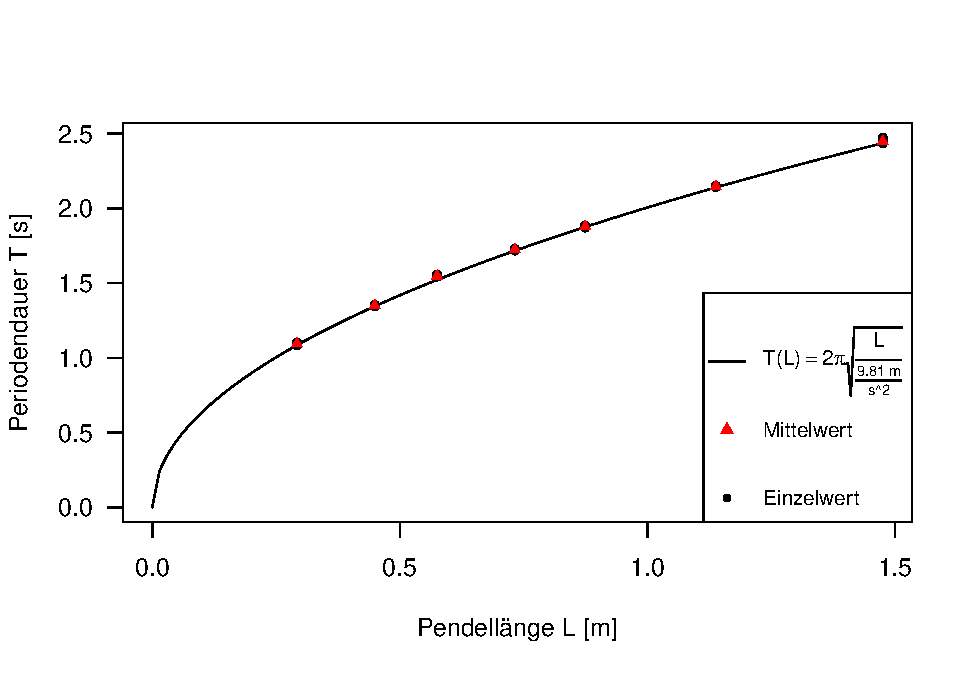
\includegraphics{Pendel_files/figure-latex/unnamed-chunk-8-1.pdf}

In diesem Diagramm sind die Fehlerbalken nicht sichtbar, was an den
kleinen Fehlern liegt. Als ersatz wurde zur Validierung der Messwerte
die Funktion \(T(L)=2\pi\sqrt{\frac{L}{g}}\) mit dem Literaturwert der
Erdbeschleunigung für Berlin von \(g\approx 9,81\frac{m}{s^2}\)
eingezeichnet. Daran wird ersichtlich, dass die Messwerte alles in allem
ganz gut sind.

\hypertarget{linearisierung}{%
\subsubsection{Linearisierung}\label{linearisierung}}

Mittels einer Linearisierung erfolgt die Berechnung von \(g\) für diesen
Versuch. Quadrierung von Formel \ref{Pendel:Periodendauer} ergibt:
\[T^2 = 4\pi^2\frac{L}{g}\] Daraus folgt eine Geradengleichung der Form
\(T^2(L)=:k(L)=a*L+y\) mit der Steigung \(a=\frac{4\pi^2}{g}\) und dem
y-Achsenabschnitt \(y\). Nach der Quadrierung der Messwerte für \(T\)
kann eine lineare Regression durchgeführt werden. Eine Prüfung der
Korellation liefert einen Korrelationskoeffizient von \(0,9998\).

\begin{Shaded}
\begin{Highlighting}[]
\CommentTok{\# Berechnung der linearisierten Funktionswerte}
\NormalTok{xlin}\OtherTok{=}\NormalTok{WerteT}\SpecialCharTok{$}\NormalTok{Pendellaenge\_L}\SpecialCharTok{/}\DecValTok{100} \CommentTok{\# in m}
\NormalTok{ylin}\OtherTok{=}\NormalTok{(WerteT}\SpecialCharTok{$}\StringTok{\textasciigrave{}}\AttributeTok{10{-}Perioden\_Mittelwert}\StringTok{\textasciigrave{}}\SpecialCharTok{/}\DecValTok{10}\NormalTok{)}\SpecialCharTok{**}\DecValTok{2} \CommentTok{\# in s}
\CommentTok{\# Korellationskoeffizient}
\FunctionTok{cor}\NormalTok{(}\AttributeTok{x=}\NormalTok{xlin, }\AttributeTok{y=}\NormalTok{ylin, }\AttributeTok{method=}\StringTok{\textquotesingle{}pearson\textquotesingle{}}\NormalTok{)}
\end{Highlighting}
\end{Shaded}

\begin{verbatim}
## [1] 0.9998811
\end{verbatim}

Die lineare Regression erfolgt in R mittels QR-Faktorisierung in der
lm()-Funktion.

\begin{Shaded}
\begin{Highlighting}[]
\FunctionTok{lm}\NormalTok{(ylin}\SpecialCharTok{\textasciitilde{}}\NormalTok{xlin)}
\end{Highlighting}
\end{Shaded}

\begin{verbatim}
## 
## Call:
## lm(formula = ylin ~ xlin)
## 
## Coefficients:
## (Intercept)         xlin  
##     0.01952      4.04209
\end{verbatim}

Im folgenden Schaubild ist die Funktionsgerade der linearen Regression
zusehen. Dabei ist die Steigung \(a=\frac{4\pi^2}{g}=4,04209\) und der
y-Achsenabschnitt \(y=0,01952\). Ebenfalls eingezeichnet sind die
quadrierten Mittelwerte Messwerten für die Periodendauer \(T\) bei den
untersuchten Pendellängen.

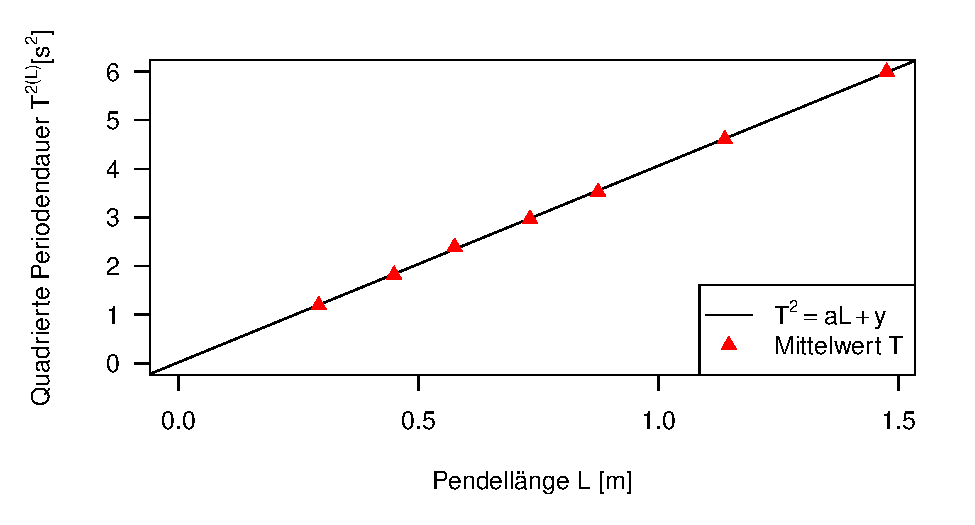
\includegraphics{Pendel_files/figure-latex/unnamed-chunk-11-1.pdf}

\hypertarget{berechnung-der-erdbeschleunigung}{%
\subsubsection{Berechnung der
Erdbeschleunigung}\label{berechnung-der-erdbeschleunigung}}

Aus der Steigung \(a\) kann die Erdbeschleunigung \(g\) bestimmt werden:

\begin{align*}
a&= \frac{4\pi^2}{g}\\
\Rightarrow g &= \frac{4\pi^2}{4,04209}\\
 &= 9,766832901879 [\frac{m}{s^2}]\\
\end{align*}

\hypertarget{weiter-mit-fehlerrechnung-g}{%
\section{Weiter mit Fehlerrechnung
g}\label{weiter-mit-fehlerrechnung-g}}

wie?

\hypertarget{todos}{%
\section{Todos:}\label{todos}}

\begin{itemize}
\tightlist
\item
  Der/Die Student/in konnte seine/ihre Messergebnisse der zwei
  Messmethoden vergleichen (5 Punkte).
\item
  Der/Die Student/in konnte beurteilen welche der beiden Methoden
  richtiger oder präziser ist (5 Punkte).
\item
  Der/Die Student/in konnte Ursachen für systematische Abweichungen bei
  den unter- schiedlichen Messmethoden finden (10 Punkte).
\item
  Rückschlüsse sind klar dargestellt und beziehen sich auf die eigenen
  Messdaten und deren Analyse (5 Punkte).
\end{itemize}

\end{document}
